\documentclass[preview]{standalone}

\usepackage{amsmath}
\usepackage{amssymb}
\usepackage{parskip}
\usepackage{fullpage}
\usepackage{hyperref}
\usepackage{tikz}
\usepackage{float}
\usepackage{xcolor}
\usepackage{stellar}
\usepackage{definitions}
\usepackage{bettelini}

\begin{document}

\id{differentiation}
\genpage

\section{Tangent lines}

%\begin{snippet}{slope-of-function-illustration}
%    \begin{minipage}{0.5\textwidth}
%        \begin{tikzpicture}[
%            scale=2,
%            declare function={
%                func(\x) = \x*sin(\x r);
%                Width=3;
%                Height=2;
%                Ax=0.75;
%                Bx=2.25;
%                SlopeMargin=0.25;
%                M=(func(Bx) - func(Ax)) / (Bx - Ax);
%                Q=func(Ax) - M * Ax;
%                slopeFunc(\x)=\x * M + Q;
%            }
%        ]
%            \draw[domain=-0.5:3, smooth, variable=\x, blue, very thick] plot ({\x}, {func(\x)});
%            
%            \draw[->] (0, -0.25) -- (0, Height) node[right] {\(y\)};
%            \draw[->] (-0.25, 0) -- (Width, 0) node[above] {\(x\)};
%
%            \draw[-] (Ax, {func(Ax)}) -- node[below] {\(\Delta x\)} (Bx, {func(Ax)});
%            \draw[-] (Bx, {func(Ax)}) -- node[right] {\(\Delta y\)} (Bx, {func(Bx)});
%            
%            \filldraw [red, thick] ({Ax - SlopeMargin}, {slopeFunc(Ax - SlopeMargin)}) -- ({Bx + SlopeMargin}, {slopeFunc(Bx + SlopeMargin)});
%            
%            \filldraw (Ax,{func(Ax)}) circle (1pt) node[above left] {\(A\)};
%            \filldraw (Bx,{func(Bx)}) circle (1pt) node[above] {\(B\)};
%        \end{tikzpicture}
%    \end{minipage}
%    \begin{minipage}{0.5\textwidth}
%        The mean slope of a \function \(f\) between a point \(A\) and \(B\) is given by
%        \[
%            \frac{\Delta y}{\Delta x} = \frac{f(B)-f(A)}{B-A}
%        \]
%        As we make \(A\) and \(B\) closer to each other, \(\Delta x\) decreases.
%        As \(\Delta x\) decreases the mean slope is more representative of the rate of change
%        of \(f\) in the interval \([A;B]\). \\
%    \end{minipage}
%\end{snippet}

\begin{snippet}{slope-of-function-expl}
        The mean slope of a \function \(f\) between a point \(A\) and \(B\) is given by
        \[
            \frac{\Delta y}{\Delta x} = \frac{f(B)-f(A)}{B-A}
        \]
        As we make \(A\) and \(B\) closer to each other, \(\Delta x\) decreases.
        As \(\Delta x\) decreases the mean slope is more representative of the rate of change
        of \(f\) in the interval \([A;B]\).
\end{snippet}

\includesnpt{secant-illustration}

\begin{snippet}{tangent-illustration}
    \begin{minipage}{0.5\textwidth}
        When \(\Delta x\) of the slope is infinitely small, we have the precise slope of a given point
        on the function. This slope is represented by the tangent line, which is parallel to the given point.
        \[
            \lim_{\Delta x \to 0} \frac{\Delta y}{\Delta x}
        \]
    \end{minipage}
    \begin{minipage}{0.5\textwidth}
        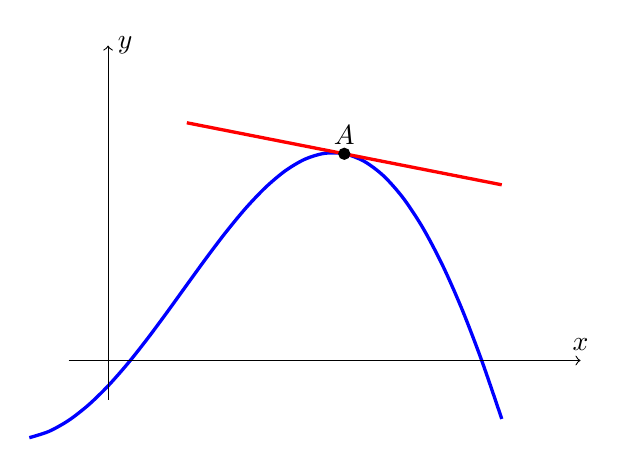
\begin{tikzpicture}[
            scale=2,
            declare function={
                func(\x) = (\x+0.6)*sin((\x+0.6) r)-0.5;
                Width=3;
                Height=2;
                Ax=1.5;
                slope = -0.19697;
            }
        ]
            \draw[domain=-0.5:2.5, smooth, variable=\x, blue, very thick] plot ({\x}, {func(\x)});
            
            \draw[->] (0, -0.25) -- (0, Height) node[right] {\(y\)};
            \draw[->] (-0.25, 0) -- (Width, 0) node[above] {\(x\)};

            \draw[domain=0.5:2.5, smooth, variable=\x, red, very thick] plot ({\x}, {slope * \x + func(Ax) - slope * Ax});
            
            \filldraw (Ax,{func(Ax)}) circle (1pt) node[above] {\(A\)};
        \end{tikzpicture}
    \end{minipage}
\end{snippet}

\section{Derivative}

\begin{snippet}{derivative-explanation}
The derivative of a \function \(f(x)\) is another \function \(f'(x)\) which
represents the rate of change of \(f(x)\). In other words, \(f'(x)\)
represents the slope at each \(x\) of \(f(x)\).
\end{snippet}

\begin{snippet}{derivative-illustration}
We define \(f'(x)\) by taking the limit of the slope for every \(x\).

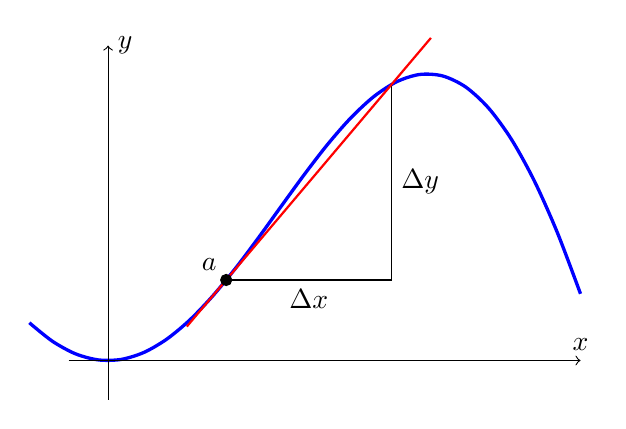
\begin{tikzpicture}[
    scale=2,
    declare function={
        func(\x) = \x*sin(\x r);
        Width=3;
        Height=2;
        Ax=0.75;
        Bx=1.8;
        SlopeMargin=0.25;
        M=(func(Bx) - func(Ax)) / (Bx - Ax);
        Q=func(Ax) - M * Ax;
        slopeFunc(\x)=\x * M + Q;
    }
]
    \draw[domain=-0.5:3, smooth, variable=\x, blue, very thick] plot ({\x}, {func(\x)});
    
    \draw[->] (0, -0.25) -- (0, Height) node[right] {\(y\)};
    \draw[->] (-0.25, 0) -- (Width, 0) node[above] {\(x\)};

    \draw[-] (Ax, {func(Ax)}) -- node[below] {\(\Delta x\)} (Bx, {func(Ax)});
    \draw[-] (Bx, {func(Ax)}) -- node[right] {\(\Delta y\)} (Bx, {func(Bx)});
    
    \filldraw [red, thick] ({Ax - SlopeMargin}, {slopeFunc(Ax - SlopeMargin)}) -- ({Bx + SlopeMargin}, {slopeFunc(Bx + SlopeMargin)});

    \filldraw (Ax,{func(Ax)}) circle (1pt) node[above left] {\(a\)};
\end{tikzpicture}
\end{snippet}

\begin{snippetdefinition}{derivative-definition}{Derivative}
    The \textit{derivative} of a \function \(f(x)\) is defined as
    \[
        f'(x) = \lim_{\Delta x \to 0} \frac{f(x + \Delta x) - f(x)}{\Delta x}
    \]
\end{snippetdefinition}

\plain{An equivalent form of the derivative is the following}
\begin{snippet}{derivative-alternate-form}
    \[
        f'(x) = \lim_{h \to x} \frac{f(h) - f(x)}{x-h}
    \]
\end{snippet}

Using the derivative, the tangent line at \(x=a\) is given by
\[
    y=f'(a)(x-a) + f(a)
\]

\section{Differentials}

\begin{snippetdefinition}{differentials-definition}{Differentials}
    Given a \function \(y = f(x)\) we call \(dy\) and \(dx\) differentials and their relationship is
    \[
        dy=f'(x)dx
    \]
    If we are given just \(f(x)\) then the differentials would be \(df\) and \(dx\)
    \[
        df = f'(x)dx
    \]
\end{snippetdefinition}

\section{Continuity class}

\begin{snippetdefinition}{continuity-class-definition}{Continuity class}
    The \emph{continuity class} is defined as
    \[
        C^n = \begin{cases}
            \{ f \colon I \to \realnumbers \suchthat f \text{ is continuous in } I \} & n = 0 \\
            \{ f \colon I \to \realnumbers \suchthat \exists f^{(n)} \text{ in } I \land \forall k \leq n, f^{(n)} \text{ is continuous in } I \} & n \in \naturalnumbers^* \\
            \{ f \colon I \to \realnumbers \suchthat \exists f^{(n)} \text{ in } I \land f^{(n)} \text{ continuous in } I \} & n = \infty
        \end{cases}
    \]
\end{snippetdefinition}

\begin{snippetproposition}{continuity-class-intersection}{Continuity class intersection}
    \[
        \continuityclass^\infty(I) = \bigcap_{n=0}^\infty \continuityclass^n(I)
    \]
\end{snippetproposition}

\end{document}